%=====================================================================
\section{What we did, in order}
%=====================================================================
The work happened in six sessions. Each one started by checking a fingerprint (a SHA-256 hash) of the code we were handed, so that we never built on the wrong version.

\subsection*{Session 1: audit and repair}
\begin{itemize}
\item \textbf{Checked the physics.} We compared the code's equations against the published PDF and the arXiv \LaTeX{} source. They matched.
Several suspected misprints we had been warned about (a square root in Eq.~3, an extra $L^2$ in Eq.~8, $\Flex=2500$ in a caption) turned out to be artefacts of copying text out of the PDF, not real misprints.
\item \textbf{Found the zero-reset bug} and fixed it, test first (Section~\ref{sec:b-bug}).
\item \textbf{Worked out which end leads} and translated the bead numbering (Section~\ref{sec:b-railway}).
\item \textbf{Built the measuring tools}, each with a test: railway MSD, rotation, structure factor, histogram, plateau finder.
\item \textbf{Ran a smoke test} (a quick ``does it switch on?'' run). Over 4000 steps at $\Pe=200$ the filament's centre moved 0.127 bead lengths and was never reset to zero, and $\spn$ stayed below 0.14.
A longer 2-million-step check at $\Pe=1000$ showed railway motion: the relative-MSD dips appeared near the predicted times (at lag 14.8 for $i=1$, predicted 10; 21.9 for $i=2$, predicted 20; 40.2 for $i=4$, predicted 40).
\end{itemize}

\subsection*{Session 2: pictures}
We built a visualizer: films of the saved snapshots, with no invented in-between frames, plus summary panels. All three Figure-2 settings were run for 100 time units each.
None formed a spiral. That was expected: 100 time units is only half a contour length even at the fastest setting.
\begin{figure}[H]\centering
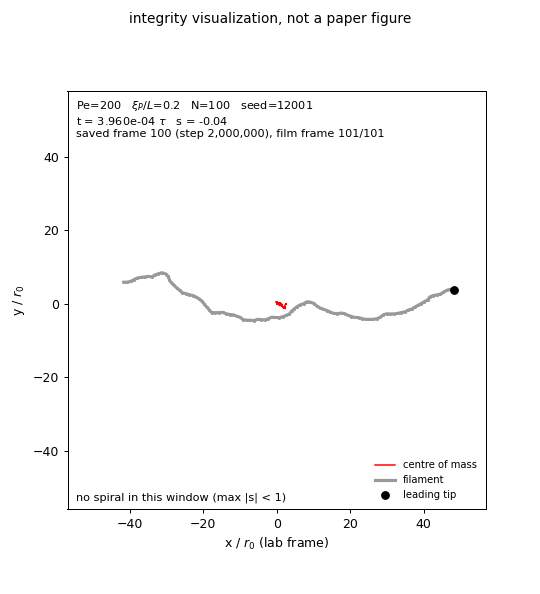
\includegraphics[width=0.38\linewidth]{frame_viz_polymer_last.png}\hspace{1em}
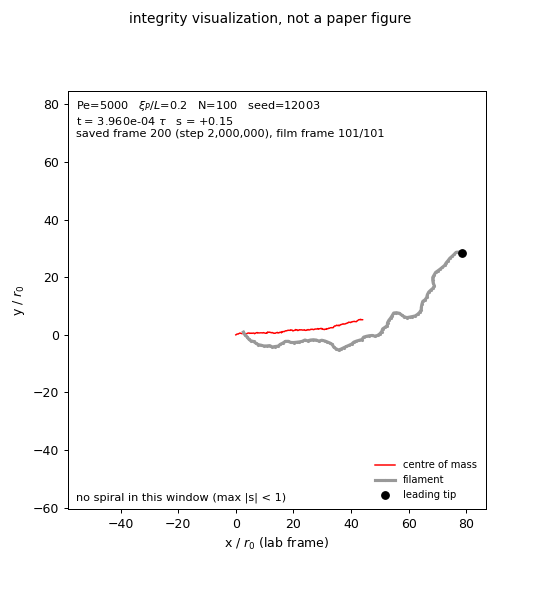
\includegraphics[width=0.38\linewidth]{frame_viz_strong_last.png}
\caption{Last frames of the session-2 films: $\Pe=200$ (left) and $\Pe=5000$ (right) after 100 time units. Grey filament, black head, red centre-of-mass trail. Too short for a spiral.}
\end{figure}

\subsection*{Session 3: the formation test (``gate'') and a mistake}
Before spending days on one long run, we ran a cheap test: does a spiral form within 10 contour lengths (about 5 minutes of computing)?
The pass rule: $|\spn|>2$ held for at least 2 contour lengths, and the centre-of-mass bookkeeping intact.
\begin{itemize}
\item Seed 12013 with the \code{paper_all_pairs} policy passed: a spiral at $\spn\approx-4.1$ for 3.8 contours.
\item Seed 12003 with \code{lammps_default} failed.
\end{itemize}
We then started a long run, but with the \emph{wrong} seed (12003, never shown to spiral under that policy) and with snapshots too far apart (one every 12.5 contours, longer than the whole spiral we had seen). It was stopped and never used.

\subsection*{Session 4: untangling seed from policy}
The first gate changed two things at once, the policy \emph{and} the seed, so we crossed them:
\begin{figure}[H]\centering
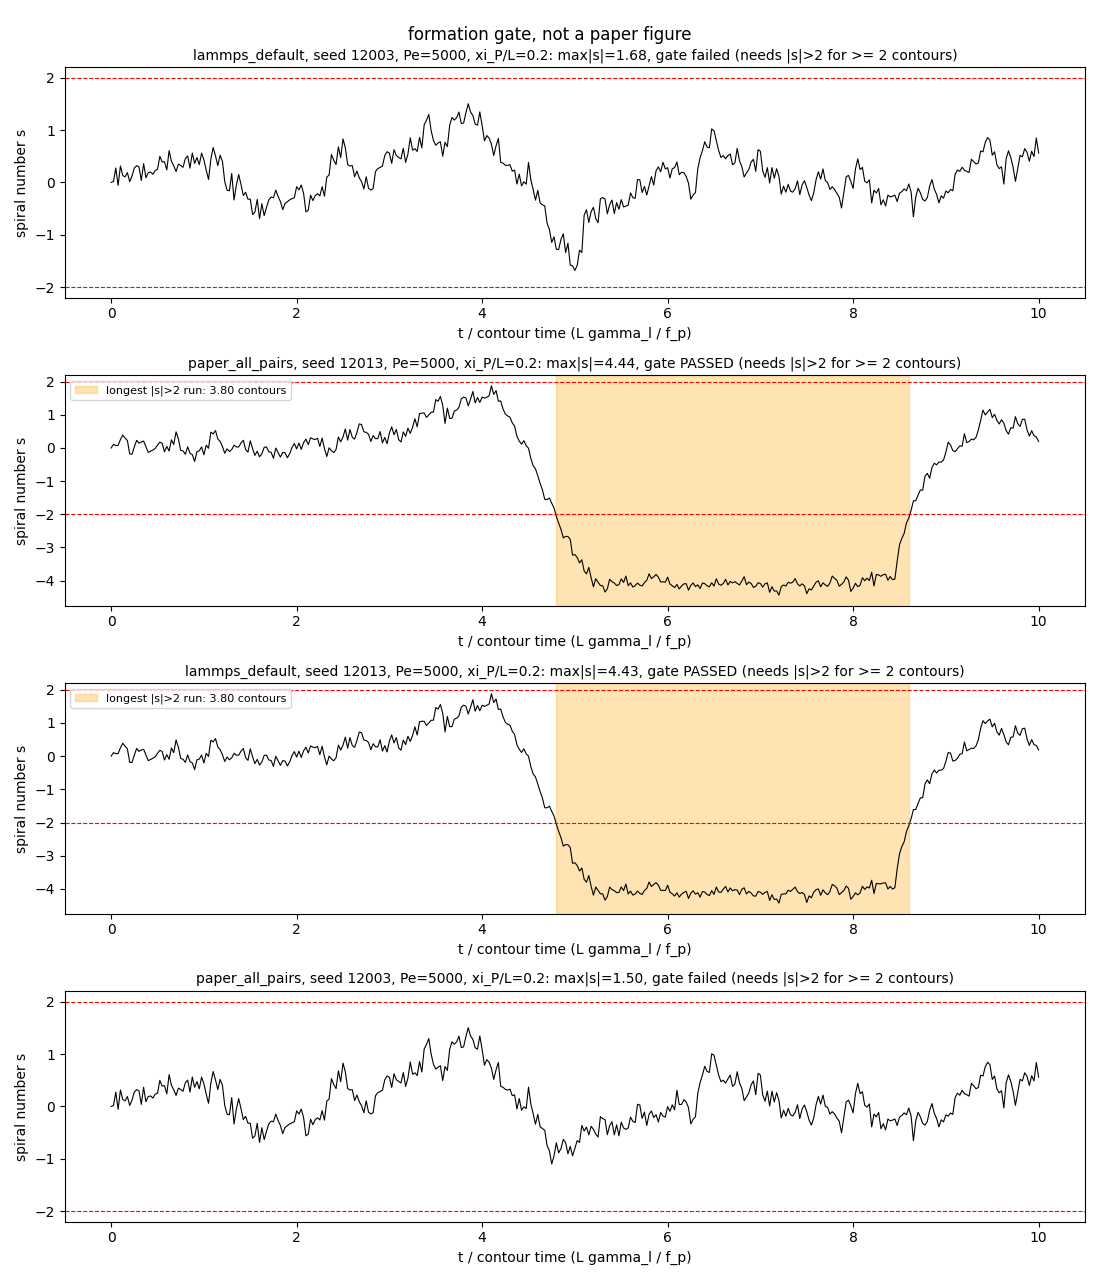
\includegraphics[width=0.78\linewidth]{gate4_s_t.png}
\caption{The four gate runs (10 contours each). Seed 12013 winds up under \emph{both} policies; seed 12003 under \emph{neither}. The random seed decided, not the policy.}
\end{figure}
Why did the seed matter more than the policy? With the same seed, both runs receive identical random kicks. The two policies differ only for beads at most 3 apart along the chain, while
spirals form when beads far apart touch. So the runs stay almost identical. The lesson: change one thing at a time.

We also built the tools for the long run:
\begin{itemize}
\item snapshots every 0.25 contour, so a 3.8-contour spiral spans about 15 frames;
\item a \code{--seed} option;
\item the segment stitcher;
\item a zoomed film of the spiral.
\end{itemize}
\begin{figure}[H]\centering
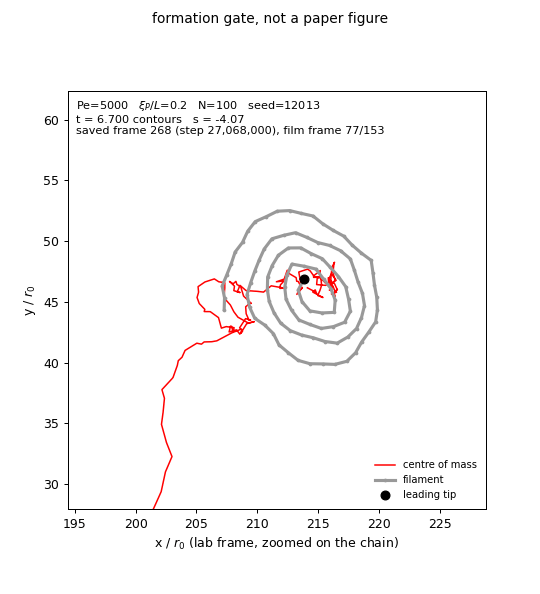
\includegraphics[width=0.42\linewidth]{frame_gate_plateau.png}
\caption{Zoom on the wound filament in the gate run: about four turns, head (black) in the centre, centre of mass (red) wandering.}
\end{figure}
Then the long run began: seed 12013, \code{paper_all_pairs}, $5\tau$.

\subsection*{Session 5: writing the verdict before the answer}
While the run went on, we wrote and tested the verdict program (Section~\ref{sec:b-verdict}), including fake data for each description and a refusal test for a too-short file.

\subsection*{Session 6: interruption, rescue, finish}
\begin{itemize}
\item \textbf{The crash.} Two hours in, at step 862\,540\,000 (3.4\% done), the process silently stopped. Fourteen seconds later Windows logged an update of the Claude application, which had launched the job, so the update most likely took the job down with it.
\item \textbf{Nothing was lost.} The checkpoint was intact, and so was the saved data (855 snapshots).
\item \textbf{Restarted from your own session.} Our assistant was not allowed to start long background jobs or change its own permissions, so you started the resume by double-clicking a prepared script. That also made the job independent of the app.
\item \textbf{The finish.} It ran 53 more hours at about 127\,000 steps per second and finished on 5 October 2026 at 06:03. We stitched the two pieces, ran the verdict, and drew the figures.
\end{itemize}

%=====================================================================
\section{What we found, explained}
%=====================================================================
\begin{figure}[H]\centering
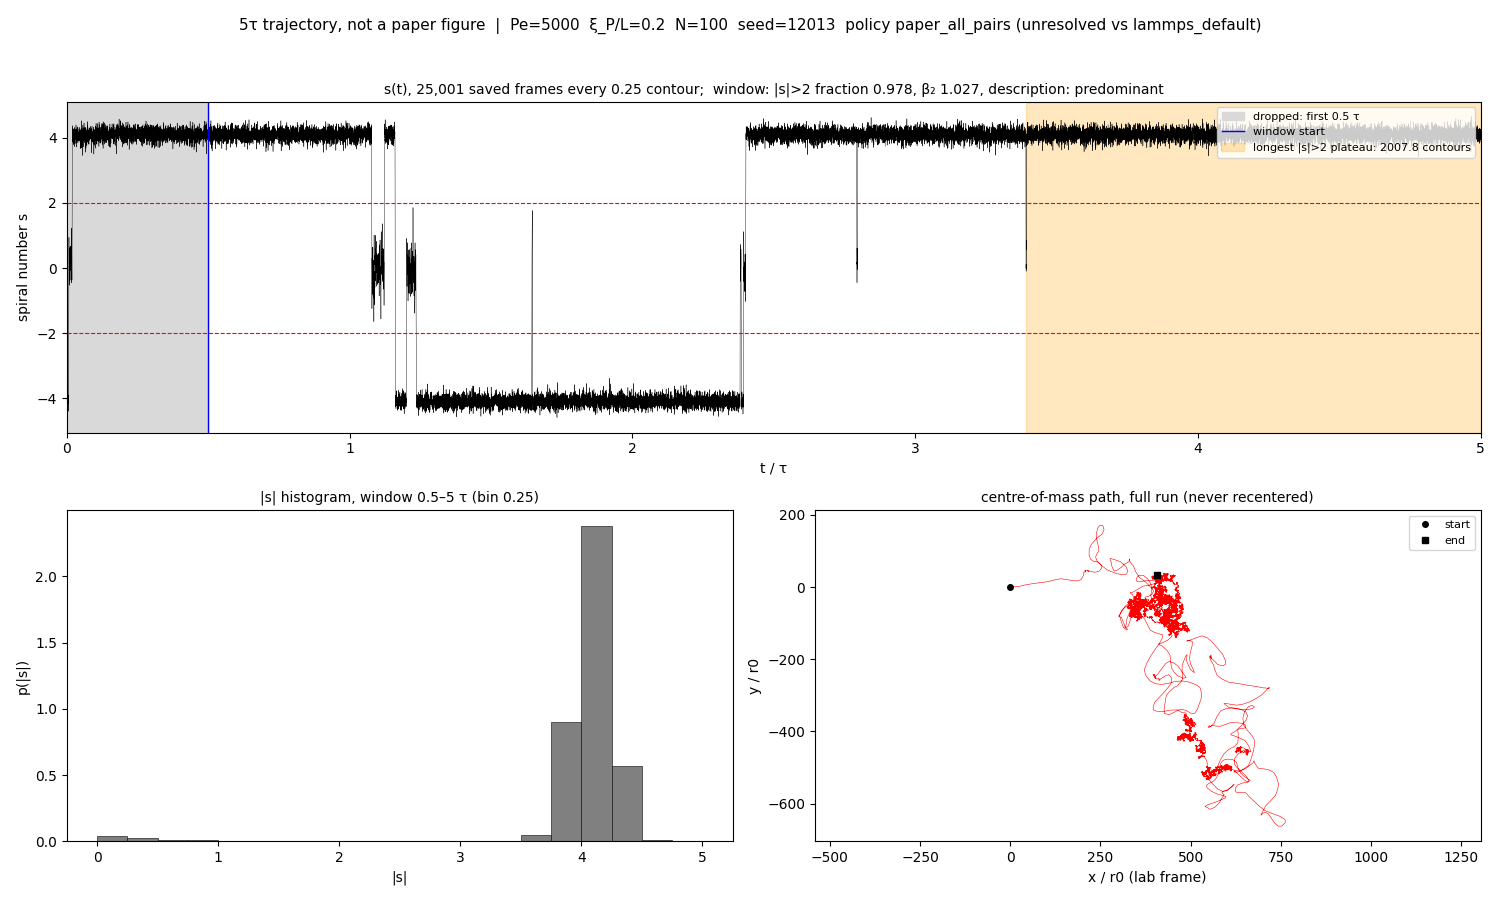
\includegraphics[width=\linewidth]{result_panel.png}
\caption{The finished $5\tau$ run. Top: the spiral number over time; grey is the start-up period we ignore, orange the longest unbroken spiral. Bottom left: how often each $|\spn|$ value occurred. Bottom right: the path of the centre of mass.}
\end{figure}

\begin{center}
\begin{tabular}{p{0.38\linewidth}p{0.18\linewidth}p{0.36\linewidth}}\toprule
measured (after the first $0.5\tau$) & value & meaning\\ \midrule
time with $|\spn|>2$ & 97.8\% & almost always wound up\\
$\beta_2$ & 1.03 & two sharp peaks at $\pm4$: spiral-dominated\\
longest unbroken spiral & $\geq2007.75$ contours & still intact when the run ended\\
centre-of-mass MSD slope & 1.00 & while wound, it drifts randomly instead of travelling\\
rotation slope-1 region & none & so no $D_r$ is reported\\
\textbf{description} & \textbf{predominant} & fraction $>1/2$ and $\beta_2<2$\\ \bottomrule
\end{tabular}
\end{center}

\textbf{Reading the top panel.}
\begin{itemize}
\item A spiral forms almost immediately and holds at $\spn\approx+4$ until about $1.1\tau$.
\item It breaks up briefly, then re-forms the other way round ($\spn\approx-4$) until about $2.4\tau$.
\item It flips back to $+4$ and stays there to the end.
\item A few single-snapshot dips are visible.
\end{itemize}
So spirals here do break and re-form; they are not permanent.

\textbf{Reading the histogram.} 97.7\% of snapshots have $|\spn|$ between 3.5 and 4.75, and only about 2\% are below 1. A tiny peak for ``stretched out'' and a huge peak for ``wound'' is the shape the paper describes for its strong-spiral example.

\textbf{Reading the path.} Dense tangles appear where the spiral spun in place and drifted randomly, linked by long straight stretches where the filament was unwound and crawling. The paper's Figure~2 caption describes exactly these ``separated clusters''.

\begin{figure}[H]\centering
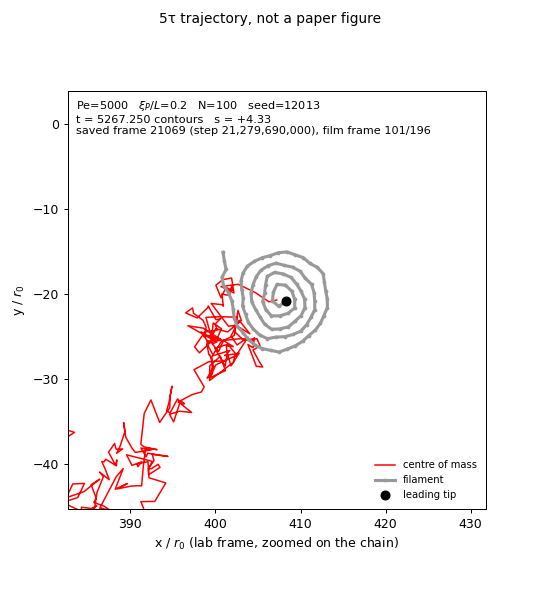
\includegraphics[width=0.42\linewidth]{frame_result_plateau.png}
\caption{A frame from the film of the longest spiral: four tight turns, head at the centre. The view follows the filament as it drifts.}
\end{figure}

%=====================================================================
\section{Is this a reproduction of the paper? Not yet}
%=====================================================================
\begin{warnbox}[title=Why ``agrees with the paper'' is not the same as ``reproduced the paper'']
\begin{itemize}
\item \textbf{One random seed.} Another seed (12003) did not even wind up in the first 10 contours. We do not know how typical our run is.
\item \textbf{One of three settings.} The polymer ($\Pe=200$) and weak-spiral ($\Pe=1000$) runs at full length have not been done.
\item \textbf{Unknown inputs.} The timestep and the repulsion setting are not published. Both could shift break-up rates.
\item \textbf{No numbers compared yet.} We compared shapes and descriptions, not values read off the paper's plots.
\item \textbf{Most figures untouched.} The motion figures (6, 8, 9, 10) and the phase diagram (Figure 4e) have not been computed at full length.
\end{itemize}
\end{warnbox}
In the project's six-stage ladder:
\begin{enumerate}
\item force law: done;
\item measuring tools: done;
\item spiral formation: partly done;
\item one long strong-spiral run: done, for one seed;
\item the other settings and the motion figures: not started;
\item the phase diagram: blocked on the missing inputs.
\end{enumerate}

%=====================================================================
\section{A tour of the code}
%=====================================================================
Everything lives in the folder \code{spin-chain-paper-v2/spin-chain-paper-v2}. The simulator is the Python package \code{src/spinchain}; the heavy number-crunching is compiled to machine code by \emph{Numba}.

\begin{figure}[H]\centering
\begin{tikzpicture}[node distance=0.55cm and 0.6cm,box/.style={draw,rounded corners,fill=boxblue,align=center,font=\footnotesize,minimum height=0.9cm,text width=2.75cm},arr/.style={-{Stealth},thick}]
\node[box] (par) {\code{parameters.py}\\ \code{paper.py}\\ settings};
\node[box,right=of par] (eng) {\code{engine.py}, \code{rng.py}\\ move the beads};
\node[box,right=of eng] (sim) {\code{simulator.py}\\ run, save, checkpoint};
\node[box,right=of sim] (h5) {\code{io.py}\\ trajectory file (\code{.h5})};
\node[box,below=1.1cm of h5] (st) {\code{stitch.py}\\ join segments};
\node[box,left=of st] (an) {\code{analysis.py}\\ \code{observables.py}\\ measure};
\node[box,left=of an] (vd) {\code{tests/verdict.py}\\ judge the run};
\node[box,left=of vd] (vz) {\code{visualize.py}\\ films and panels};
\draw[arr] (par)--(eng); \draw[arr] (eng)--(sim); \draw[arr] (sim)--(h5); \draw[arr] (h5)--(st); \draw[arr] (st)--(an); \draw[arr] (an)--(vd); \draw[arr] (an)--(vz);
\node[above=0.2cm of sim,font=\small] {\code{cli.py}: the commands you type};
\end{tikzpicture}
\caption{How data flows through the code: settings, simulation, file, then stitching, measurement, verdict and pictures.}
\end{figure}

\begin{longtable}{p{0.27\linewidth}p{0.66\linewidth}}\toprule file & in plain words\\ \midrule\endhead
\code{parameters.py} & Turns $\Pe$ and $\xiP/L$ into actual forces and stiffness, refuses unsafe timesteps, and makes a fingerprint of the settings so files cannot be mixed up.\\
\code{paper.py} & The three Figure-2 settings (polymer, weak, strong) and their default seeds.\\
\code{rng.py} & The replayable random-number generator.\\
\code{forces.py} & A slow but simple force calculation used to check the fast one.\\
\code{engine.py} & The fast stepping routine with the neighbour list. (The old zero-reset is off and can only be switched on with bookkeeping.)\\
\code{simulator.py} & The loop: step, save a snapshot, flush, checkpoint, track the end-to-end angle.\\
\code{io.py} & Writes the trajectory file and labels it (origin, policy, timestep status).\\
\code{checkpoint.py} & Saves and reloads the exact state; refuses a checkpoint from different settings.\\
\code{observables.py} & The measuring tools: spiral number, kurtosis, MSDs, rotation, structure factor, plateau finder.\\
\code{analysis.py} & Reads a file and computes the paper's quantities over a window you choose.\\
\code{stitch.py} & Joins segments, refusing gaps, overlaps or mismatched starts.\\
\code{visualize.py} & Films and panels from saved snapshots only.\\
\code{cli.py} & The commands: \code{benchmark}, \code{headless}, \code{paper-reproduce}, \code{analyze}, \code{visualize}, and more.\\
\code{tests/} & 64 automatic tests, plus helper scripts: \code{smoke_integrity.py}, \code{formation_gate.py}, \code{verdict.py}, \code{result_figures.py}.\\
\code{output/} & Everything the runs produced: gate runs, films, the long run, verdict, figures.\\
\code{*.md} notes & One note per session, from \code{REPRO_NOTE.md} to \code{RESULT_NOTE.md}.\\ \bottomrule
\end{longtable}

\textbf{What is inside a trajectory file?}
\begin{itemize}
\item One row per saved snapshot: the step number, the time (in simulation units and in $\tau$), $\spn$, the centre of mass, the end-to-end vector and its counted-turns angle, the size of the coil, and all 101 bead positions.
\item Labels saying where the origin is, which end leads, which policy was used, and that the timestep is unpublished.
\item A ``complete'' flag that is true only if the run reached its target.
\end{itemize}

%=====================================================================
\section{How to run it yourself}
%=====================================================================
\subsection{One-time setup (Windows)}
Open a terminal in the folder \texttt{spin-chain-paper-v2\textbackslash spin-chain-paper-v2} and type:
\begin{lstlisting}[style=sh]
uv venv -p 3.11 .venv311
uv pip install -p .venv311/Scripts/python.exe -r requirements.txt
set PYTHONPATH=src
.venv311\Scripts\python.exe -m pytest -q
\end{lstlisting}
The last line should end with ``64 passed''. (\code{uv} is a fast Python installer. With ordinary Python, create a 3.11 environment and run \code{pip install -r requirements.txt}.)
In every new terminal, run \code{set PYTHONPATH=src} again, or use the full commands below.

\subsection{Recipe 1: how fast is my computer?}
\begin{lstlisting}[style=sh]
.venv311\Scripts\python.exe -m spinchain benchmark --regime strong_spiral --policy paper_all_pairs --steps 20000
\end{lstlisting}
Read \code{steps_per_second}. Then $2.525\times10^{10}$ divided by that number gives the seconds for a $5\tau$ run.

\subsection{Recipe 2: a quick look (minutes)}
\begin{lstlisting}[style=sh]
.venv311\Scripts\python.exe -m spinchain headless --regime strong_spiral --steps 2000000 --sample-every 10000 --output output/viz/try.h5 --overwrite
.venv311\Scripts\python.exe -m spinchain visualize output/viz/try.h5
\end{lstlisting}
This writes \code{output/viz/try.gif} (a film) and \code{try.png} (a panel). It is far too short for spirals; it is just a look.

\subsection{Recipe 3: the formation gate (about 5 minutes per run)}
\begin{lstlisting}[style=sh]
.venv311\Scripts\python.exe -m spinchain headless --regime strong_spiral --policy paper_all_pairs --steps 40400000 --sample-every 101000 --output output/gate/my-gate.h5 --overwrite
.venv311\Scripts\python.exe tests/formation_gate.py --name mygate output/gate/my-gate.h5
\end{lstlisting}
Ten contours at $\Pe=5000$ is 40\,400\,000 steps. The script prints whether the gate passed and draws \code{mygate_s_t.png}.

\subsection{Recipe 4: a full $5\tau$ run (about 2.5 days)}
\begin{warnbox}[title=Start long runs yourself]
Start long runs from your own terminal or by double-clicking a script, \emph{not} from inside the AI assistant. A job started by the app can be killed when the app updates, which is exactly what happened to us. Keep the window open, keep the laptop plugged in, and use the ``Best performance'' power mode.
\end{warnbox}
\begin{lstlisting}[style=sh]
.venv311\Scripts\python.exe -m spinchain paper-reproduce --regime strong_spiral --policy paper_all_pairs --seed 12013 --tau 5 --replicates 1 --output-dir output/reproduction/my-run --i-know
\end{lstlisting}
\begin{itemize}
\item \textbf{Watch progress} by looking at the last lines of the log (\code{progress: step=... tau=...}). Do \emph{not} open the \code{.h5} file while it is being written.
\item \textbf{If it stops,} run the same command with \code{--resume} added. It picks up from the last checkpoint and writes a new segment file.
\item \textbf{It is finished} when the log ends with \code{"completed": true}.
\end{itemize}

\subsection{Recipe 5: stitch, judge, draw}
\begin{lstlisting}[style=sh]
.venv311\Scripts\python.exe -c "import glob;from spinchain.stitch import write_stitched;print(write_stitched(glob.glob('output/reproduction/my-run/strong_spiral-seed12013*.h5'),'output/reproduction/my-run-stitched.h5'))"
.venv311\Scripts\python.exe tests/verdict.py output/reproduction/my-run-stitched.h5 --out output/reproduction/my-verdict.json
.venv311\Scripts\python.exe tests/result_figures.py output/reproduction/my-run-stitched.h5 output/reproduction/my-verdict.json --out-dir output/reproduction/my-result
\end{lstlisting}

\subsection{Common problems}
\begin{description}[style=nextline]
\item[``FileExistsError''] The output file already exists. Choose a new name. Add \code{--overwrite} only if you really want to throw the old one away.
\item[``fingerprint mismatch''] You are resuming with different settings (seed, policy, $\Pe$) from the original run.
\item[The verdict says ``refused''] The run is shorter than $5\tau$, or the file is damaged or unlabelled. The message says which.
\item[A path like \code{/c/Users} creates odd folders] In Windows Python, write \code{C:/Users/...}.
\item[It is slow] Plug in, use Best performance, close heavy programs. Spiral phases run a little slower because more beads touch.
\end{description}

%=====================================================================
\section{Where to go next, and why}
%=====================================================================
\begin{enumerate}
\item \textbf{Find the missing numbers (hours).}
\begin{itemize}
\item Download the paper's supplementary file; it may list the timesteps and the simulation input.
\item Measure numbers off the paper's plots (``digitize'' them), so we can compare values, not just shapes.
\end{itemize}
\item \textbf{Run several jobs at once (about 3 days).} The laptop has 8 logical cores and each job uses one, so run together:
\begin{itemize}
\item $\Pe=200$ and $\Pe=1000$, to see all three regimes;
\item seed 12003 and one new seed at $\Pe=5000$, to test how typical our result is;
\item seed 12013 under the other policy, to see whether break-ups differ.
\end{itemize}
\item \textbf{The motion figures (6, 8, 9, 10).} These need other settings and, for Figure~6, snapshots close together.
\item \textbf{The phase diagram.} About 100--150 days of single-core computing: a project for a computing cluster, or for one slice of the diagram.
\end{enumerate}

%=====================================================================
\section{Glossary}
%=====================================================================
\begin{description}[style=nextline,itemsep=0.1em]
\item[Bead--spring model] A filament represented as beads joined by springs.
\item[Brownian motion] Random jiggling caused by molecular collisions.
\item[Checkpoint] A saved exact state from which a run can continue.
\item[Contour time] Time for the filament to crawl one body length; 202 time units at $\Pe=5000$.
\item[Euler--Maruyama] The simplest correct step rule for equations with random noise.
\item[Excluded volume (WCA)] Short-range repulsion that prevents the filament crossing itself.
\item[Flexure number $\Flex$] Pushing versus stiffness; large values favour spirals.
\item[Gate] A cheap pre-test run before an expensive one.
\item[$\kT$] Thermal energy, the unit of energy here.
\item[Kurtosis $\beta_2$] A shape number: 3 for a bell curve, 1 for two sharp peaks.
\item[MSD] Mean square displacement: average squared distance moved over a time lag.
\item[Neighbour (Verlet) list] A saved list of nearby bead pairs, rebuilt only when needed.
\item[Overdamped] Friction dominates inertia: velocity is proportional to force.
\item[Péclet number] Directed motion versus diffusion.
\item[Persistence length $\xiP$] The distance over which the filament keeps its direction.
\item[Plateau] A stretch of consecutive snapshots with $|\spn|>2$.
\item[Policy] Which nearby bead pairs feel the repulsion. Unresolved, because the setting is unpublished.
\item[Railway motion] The filament sliding along its own outline.
\item[Seed] The integer that determines the whole stream of random numbers.
\item[Segment] One file of a run that was interrupted and resumed.
\item[Spiral number $\spn$] Total turning along the filament, in full turns.
\item[Stitching] Joining segments into one exact trajectory.
\item[$\tau$] The time to diffuse one's own length; $5\tau$ is the paper's run length.
\item[Verdict] Pre-written rules that describe a finished run.
\end{description}

%=====================================================================
\section{Exercises (answers below)}
%=====================================================================
\begin{enumerate}
\item With $L=100$, $\kT=1$: what is $f_p$ for $\Pe=1000$? What is the flexure number at $\xiP/L=0.2$?
\item How many steps is $5\tau$ at $\Delta t=5\times10^{-5}$, with $\tau=252\,500$? How long at 120\,000 steps/s?
\item A filament's $|\spn|$ is exactly 4 half the time and exactly 0 the other half. What is the symmetrized $\beta_2$?
\item Why does resetting the centre of mass to zero in every saved frame ruin the centre-of-mass MSD, but not the spiral number?
\item Two runs use the same seed but different policies. Why can their spiral histories look almost identical?
\item The verdict saw fraction $=0.3$ and a 5-contour plateau. Which description applies?
\item Why must the random numbers depend on (seed, step, bead) and not on ``how many numbers were drawn so far''?
\item Paper bead 25 is which code bead for $N=100$? Why is there a difference?
\end{enumerate}

\subsection*{Answers}
\begin{enumerate}
\item $f_p=1000/100^2=0.1$; $\Flex=1000/0.2=5000$.
\item $5\times252\,500/(5\times10^{-5})=2.525\times10^{10}$ steps; divided by $1.2\times10^5$ steps/s gives $2.1\times10^5$\,s, about 58 hours.
\item Values $\{\pm4,\pm4,0,0\}$ in equal proportion: the mean is 0, the variance is 8, the fourth moment is $128$, so $\beta_2=128/64=2$.
\item The MSD compares positions at different times. If every frame is shifted back to the origin, the measured displacement is only the noise inside one reset period. The spiral number depends only on the shape within a single frame, which a shift does not change.
\item Same seed means identical random kicks. The policies differ only for beads at most 3 apart, while spirals form when far-apart beads touch.
\item \emph{Intermittent}: a plateau longer than 2 contours exists and the fraction is below 1/2.
\item So a run that is split, stopped and resumed draws exactly the same numbers and reproduces the same trajectory bit for bit.
\item Code bead $101-25=76$. The paper's propulsion pushes towards bead 1 and ours towards the last bead: the same physics, numbered backwards.
\end{enumerate}

\appendix
\section{Key numbers}
\begin{center}\small
\begin{tabular}{lp{0.6\linewidth}}\toprule
beads / bonds & 101 / 100\\
$\kappa$, $k_S$, $\Delta t$ & 20, 4000, $5\times10^{-5}$ (timestep unpublished)\\
$\tau$ & 252\,500 time units ($5.05\times10^9$ steps)\\
contour time at $\Pe=5000$ & 202 time units ($4.04\times10^6$ steps)\\
long run & seed 12013, \code{paper_all_pairs}, $5\tau$, 25\,001 snapshots, about 55 h of computing\\
result & 97.8\% of the time $|\spn|>2$; $\beta_2=1.03$; longest spiral $\geq2007.75$ contours; \emph{predominant}\\ \bottomrule
\end{tabular}
\end{center}

\section{How these reports were built}
Both reports are \LaTeX{} documents in the folder \code{reports/}. The expert report is in \code{expert/} and this one in \code{beginner/}; they share the preamble \code{common/preamble.tex} and the folder \code{figures/}.
To rebuild one, run \code{pdflatex report_beginner.tex} twice in its folder. The second pass fills in the table of contents and cross-references.

\vspace{1em}
\begin{keybox}
\textbf{Take-home message.} We now have a simulator we trust, tools that measure what the paper measures, and one long run in which the filament was spiral-wound almost all the time.
That matches the paper's strong-spiral picture \emph{for this run}. To call it a reproduction, we need more seeds, the other settings, and the unpublished inputs.
\end{keybox}
